%%%%%%%%%%%%%%%%%%%%%%%%%%%%%%%%%%%%%%%%%%%%%%%%%%%%%%%%%%%%%%%%%%%%%%%%%%%%%%%%
%2345678901234567890123456789012345678901234567890123456789012345678901234567890
%        1         2         3         4         5         6         7         8

%\documentclass{article}
\documentclass[letterpaper, 10 pt, conference]{ieeeconf}  % Comment this line out
                                                          % if you need a4paper
%\documentclass[a4paper, 10pt, conference]{ieeeconf}      % Use this line for a4
                                                          % paper


\overrideIEEEmargins
% See the \addtolength command later in the file to balance the column lengths
% on the last page of the document

\usepackage[protrusion=true,expansion=true]{microtype}
\usepackage{cite}
\usepackage{graphicx}
\usepackage{hyperref}
\usepackage{url}
\graphicspath{{figs/}}
\DeclareGraphicsExtensions{.pdf,.jpg,.png}

\usepackage{ifthen}

\usepackage[utf8x]{inputenc}
\usepackage[T1]{fontenc}

\usepackage{fixme}

\usepackage{listings}
\usepackage{alltt}
\usepackage{fancyvrb}
\usepackage{flushend} % equalize the column length on last page

\newcommand{\concept}[1]{{\small \texttt{#1}}}

\newcommand{\stmt}[1]{{\footnotesize \tt $\langle$ #1\relax$\rangle$}}
%\newcommand{\stmt}[1]{{\footnotesize $\langle\stmttt#1\relax\rangle$}}
%\newcommand{\rawstmt}[1]{{\footnotesize \stmttt#1\relax}}
%\def\stmttt#1 #2 #3\relax{
%\texttt{\IfBeginWith{#1}{?}{\textbf{#1}}{#1} \IfBeginWith{#2}{?}{\textbf{#2}}{\emph{#2}} \ifthenelse {\equal{#3}{true} \OR \equal{#3}{false}}{\emph{#3}}{\IfBeginWith{#3}{?}{\textbf{#3}} {#3}}}}

%\newcommand{\setstmt}[1]{{\footnotesize [\setstmttt#1\relax]}}
%\def\setstmttt#1,#2\relax{\stmttt#1\relax, \stmttt#2\relax}


\newcommand{\ie}{{\textit{i.e.\ }}}
\newcommand{\cf}{{\textit{cf\ }}}
\newcommand{\eg}{{\textit{e.g.\ }}}


\title{\LARGE \bf
Explicit Knowledge and the Deliberative Layer: Lessons Learned
}

\author{Séverin Lemaignan and Rachid Alami\\
CNRS, LAAS, 7 avenue du Colonel Roche, F-31400 Toulouse, France\\
Univ de Toulouse, LAAS, F-31400 Toulouse, France\\
{\tt severin.lemaignan@laas.fr}, {\tt rachid.alami@laas.fr}
}

\begin{document}

\maketitle
\thispagestyle{empty}
\pagestyle{empty}


%%%%%%%%%%%%%%%%%%%%%%%%%%%%%%%%%%%%%%%%%%%%%%%%%%%%%%%%%%%%%%%%%%%%%%%%%%%%%%%%
\begin{abstract}

Over the last four years, we have been slowly ramping up explicit knowledge
representation and manipulation in the deliberative and executive layers of our
robots. Ranging from situation assessment to symbolic task planning, from
verbal interaction to event-driven execution control, we have built up a
\emph{knowledge-oriented} architecture which is now used on a daily basis on our
robots.

This article presents our design choices, the articulations between the diverse
deliberative components of the robot, and the strengths and weaknesses of this
approach. We show that explicit knowledge management is not only a convenient
tool from the software engineering point of view, but also pushes for a
different, more \emph{semantic} way to address the decision-making issue in
autonomous robots.

\end{abstract}


%%%%%%%%%%%%%%%%%%%%%%%%%%%%%%%%%%%%%%%%%%%%%%%%%%%%%%%%%%%%%%%%%%%%%%%%%%%%%%%%
\section{A Knowledge-Oriented Architecture}

\subsection{Towards the cognitive robot at LAAS}

Natural interaction and cooperation are on the (dare we say,
\emph{short-term}) agenda for the human-robot interaction community. They are
keys to the broad class of \emph{interactive manipulation problems}: several
agents agree on a (more or less implicit) joint goal that requires some sort of
cooperation to be successfully achieved. This class of problems involves both
dialogue and manipulation and they are often initially underspecified: they
require iterative and interactive resolution.

Over the last years we have focused our efforts on identifying the cognitive
prerequisites of these challenges, and giving them experimental reality on the
robots: what is required for sentences like ``Let's set the table together''
to be understood by the robot, correctly interpreted in the spatial and
temporal context of the interaction, and eventually transformed into a set of
actions.

We have chosen to tackle the challenge from several ends: human-aware
navigation and motion planning~\cite{Mainprice2011}, situation assessment
coupled with motion planning~\cite{Mainprice2012}, projection of
``mightabilities'' that anticipates what surrounding agents may
do~\cite{Pandey2011}, and the design and deployment of a pervasive
\emph{knowledge-oriented} software architecture.

The last item is the focus of this paper: what ``knowledge-oriented''
architecture means, and what its benefits and drawbacks are.

\subsection{Scope of the article}

In essence, this article portrays our use of \emph{explicit semantic
interfaces} to integrate several deliberative components into a decisional
architecture for our robots. It reports on our experience with acquiring,
managing and reusing grounded knowledge in the context of human-robot
interaction.

Unlike previous publications by the authors that introduced the deliberative
modules of our robots independently from each other, this contribution is an
account of the importance of explicit knowledge manipulation when
\emph{integrating} them into a large cognitive architecture.

While we do not present experiments in this paper, the ideas and techniques we
present all have been implemented and tested on several robots (see previously
reported experiments in~\cite{Lemaignan2010, Ros2010b, Lemaignan2011a,
Warnier2012a, Sisbot2011}). Videos presenting some of these experimental
results can be watched online at~\url{http://www.laas.fr/~slemaign}.

Also note that this paper does not provide extensive review of existing
literature. We kindly refer the reader to the aforementioned articles for
in-depth discussion of related works in the different fields of cognitive
architectures for robots.

\subsection{Article overview}

In the next section, we first introduce the deliberative layer of our robots at
the functional level. It represents what we call a \emph{knowledge-oriented}
architecture, built around a central knowledge management tool called the
OpenRobot Ontology ({\sc Oro}) server.

The following sections present each of the facets of this deliberative layer:
how knowledge is produced asynchronously from geometric reasoning, how the
robot conducts grounded multi-modal interaction with humans, how knowledge is
used by decision-making components like the robot controller or the task
planner, and finally, how our knowledge-oriented architecture enables the
implementation of specific internal cognitive processes.

We conclude the article with a discussion about the strengths and weaknesses of
such a knowledge-oriented architecture, from three perspectives: the software
architect, the AI expert and the cognitician.


\section{The LAAS deliberative layer}

Fig.~\ref{fig|archi} gives an overview of the connections between the
deliberative components of our architecture~\cite{Alami2011}.

\begin{figure*}
        \centering
        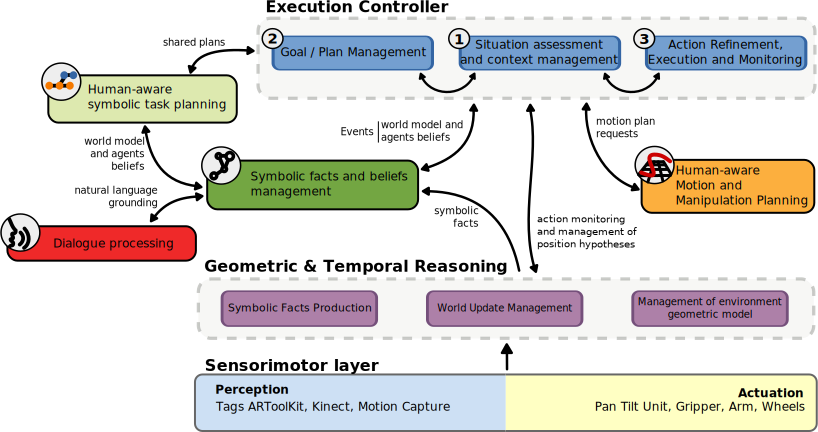
\includegraphics[width=1.7\columnwidth]{archi}
        \caption{Overview of the LAAS deliberative layer. Knowledge is
        centrally managed in an active \emph{semantic blackboard}, pictured
        above with a thick border.}
        \label{fig|archi}
\end{figure*}


This architecture moves away from standard layered approaches. Interactions
between components at the deliberative level are mostly bidirectional and we do
not introduce layers of abstraction amongst software components\footnote{We do
have lower-level modules to execute actions or manage sensors, but all
cognition-related modules reside at the same level.}. This is nicely
illustrated by the dialogue input processing. This component does not simply
act as an alternative perceptual input to the symbolic database; it also
actively queries previously acquired knowledge to disambiguate and validate the
newly created symbolic knowledge (see section~\ref{sect|com}).

Our architecture relates to \emph{Beliefs, Desires, Intentions} (BDI)
architectures. BDI architectures are primarily focused on \emph{practical
reasoning}, \ie the process of deciding, step by step, which action to perform
to reach a goal (as summarized by Woolridge~\cite{Woolridge1999}). The
management of the interaction between knowledge (the beliefs) and task and plan
representation and execution (the desires and the intentions) is central, and
aims at selecting at each step the best subgoal. It becomes then an intention
that the robot commits to.

This interaction between knowledge and actions is also central to our approach
(as for any cognitive system): it is one of the activities of the
robot, actually shared between communication components (that can acquire
desires from interaction with agents, amongst other things) and an execution
controller that may decide to take an incoming desire into account to create
its own internal goals. The controller generates and manages intentions from
these goals with the help of a symbolic task planner, that also has direct
access to the knowledge base.

This activity is however not the backbone of our architecture. Other
activities are conducted in parallel, without being explicitly considered as
desires: assessment of the situation and the environment, dialogue (including
performative dialogue that can possibly change the internal state of the robot,
but does not lead to the creation of desires, like question answering or
statement assertion), various background monitoring and recognition tasks, etc.

Regarding the anchoring question, this architecture is bidirectional. The
components we described provide a \textit{bottom-up} grounding process:
geometric reasoning and dialogue processing modules constantly build and push
new symbolic contents about the world to the knowledge base where it becomes
accessible to decisional layers. In parallel, the knowledge base relies on
reasoning in a \textit{top-down} way to produce new facts that may in return
trigger physical behaviours.

\subsection*{Knowledge model}

In our architecture (Fig.~\ref{fig|archi}), knowledge manipulation relies on a
\emph{semantic blackboard}: a central server (the {\sc Oro}
server~\cite{Lemaignan2010}) stores knowledge as it is produced by each of the
deliberative components. It conversely exposes a {\tt json}-based RPC API to
query the knowledge base~\cite{lemaignan2012kbapi}.

Knowledge is represented as RDF triples in the OWL sub-language. Each
time triples are added or removed from the knowledge base, a Description
Logics reasoner ({\sc Pellet}\footnote{\url{http://clarkparsia.com/pellet/}})
classifies the whole ontology and inserts all possible inferred triples.

Relying on RDF triples and Description Logics has advantages such as the
availability of numerous mature open-source libraries to manipulate the ontology,
interoperability with several major on-line knowledge bases (like {\sc
OpenCyc}, {\sc WordNet} or {\sc DBPedia}), open-world reasoning, and the formal
guarantee of decidability (it is always possible to classify a Description
Logics ontology).

It also has notable limitations, both fundamental (the suitability
of Description Logics when reasoning on --typically non-monotonic-- commonsense
knowledge is questionable) and practical: RDF triples imply only binary predicates
(\stmt{subject predicate object}), which constrains the expressiveness of the
system or leads to cumbersome reifications. Alternatives exist (like {\sc
KnowRob}~\cite{Tenorth2009a}) that mix RDF with more expressive logic
languages like {\sc Prolog}, at the price, however, of other limitations, like
closed-world reasoning or immutable T-Box. The classification
performance is another issue: from our experience, with an ontology sized for a
standard experiment (about 100 classes and 200 instances), classification
typically takes about 100ms, which becomes problematic during interactions.
Besides, the performances are difficult to predict, since a seemingly
inoffensive new statement may indirectly change radically the logical
complexity of the whole knowledge model and lead to notable degradation of
classification time.

This knowledge model also largely excludes representation of continuous
phenomena (like time) or uncertain phenomena. When required (for instance for
action recognition), these are managed inside the corresponding components, and
are not exposed at the semantic level.

Tools to manipulate and reason over ontologies are readily available, mature,
and already well accepted in the robotic community~\cite{Tenorth2009a,
Lim2011}. While alternatives like \emph{Answer Set Programming} have also been
successfully investigated in robotics~\cite{Chen2010,Erdem2012}, in particular
to deal with non-monotonic reasoning, we did not actually hit any brick wall
while working with OWL ontologies. We may reconsider this choice at a later
stage, but until now it has proven an effective framework to quickly explore
implementations of new cognitive abilities (for instance, it has been
conceptually and technically easy to add support for independent knowledge
models, one per the agents the robot interacts with --see
section~\ref{sect|tom}).

Besides, because ontologies and RDF statements are relatively simple concepts
to grasp, it also effectively helped to grow awareness amongst colleagues on
the significance of the ``semantic level'' when developing new components for
the robot.


%%%%%%%%%%%%%%%%%%%%%%%%%%%%%%%%%%%%%%%%%%%%%%%%%%%%%%%%%%%%%%%%%%%%%%%%%%%%%%%%
\section{Situation Assessment}
\label{sect|sit-ass}

\begin{figure}
        \centering
        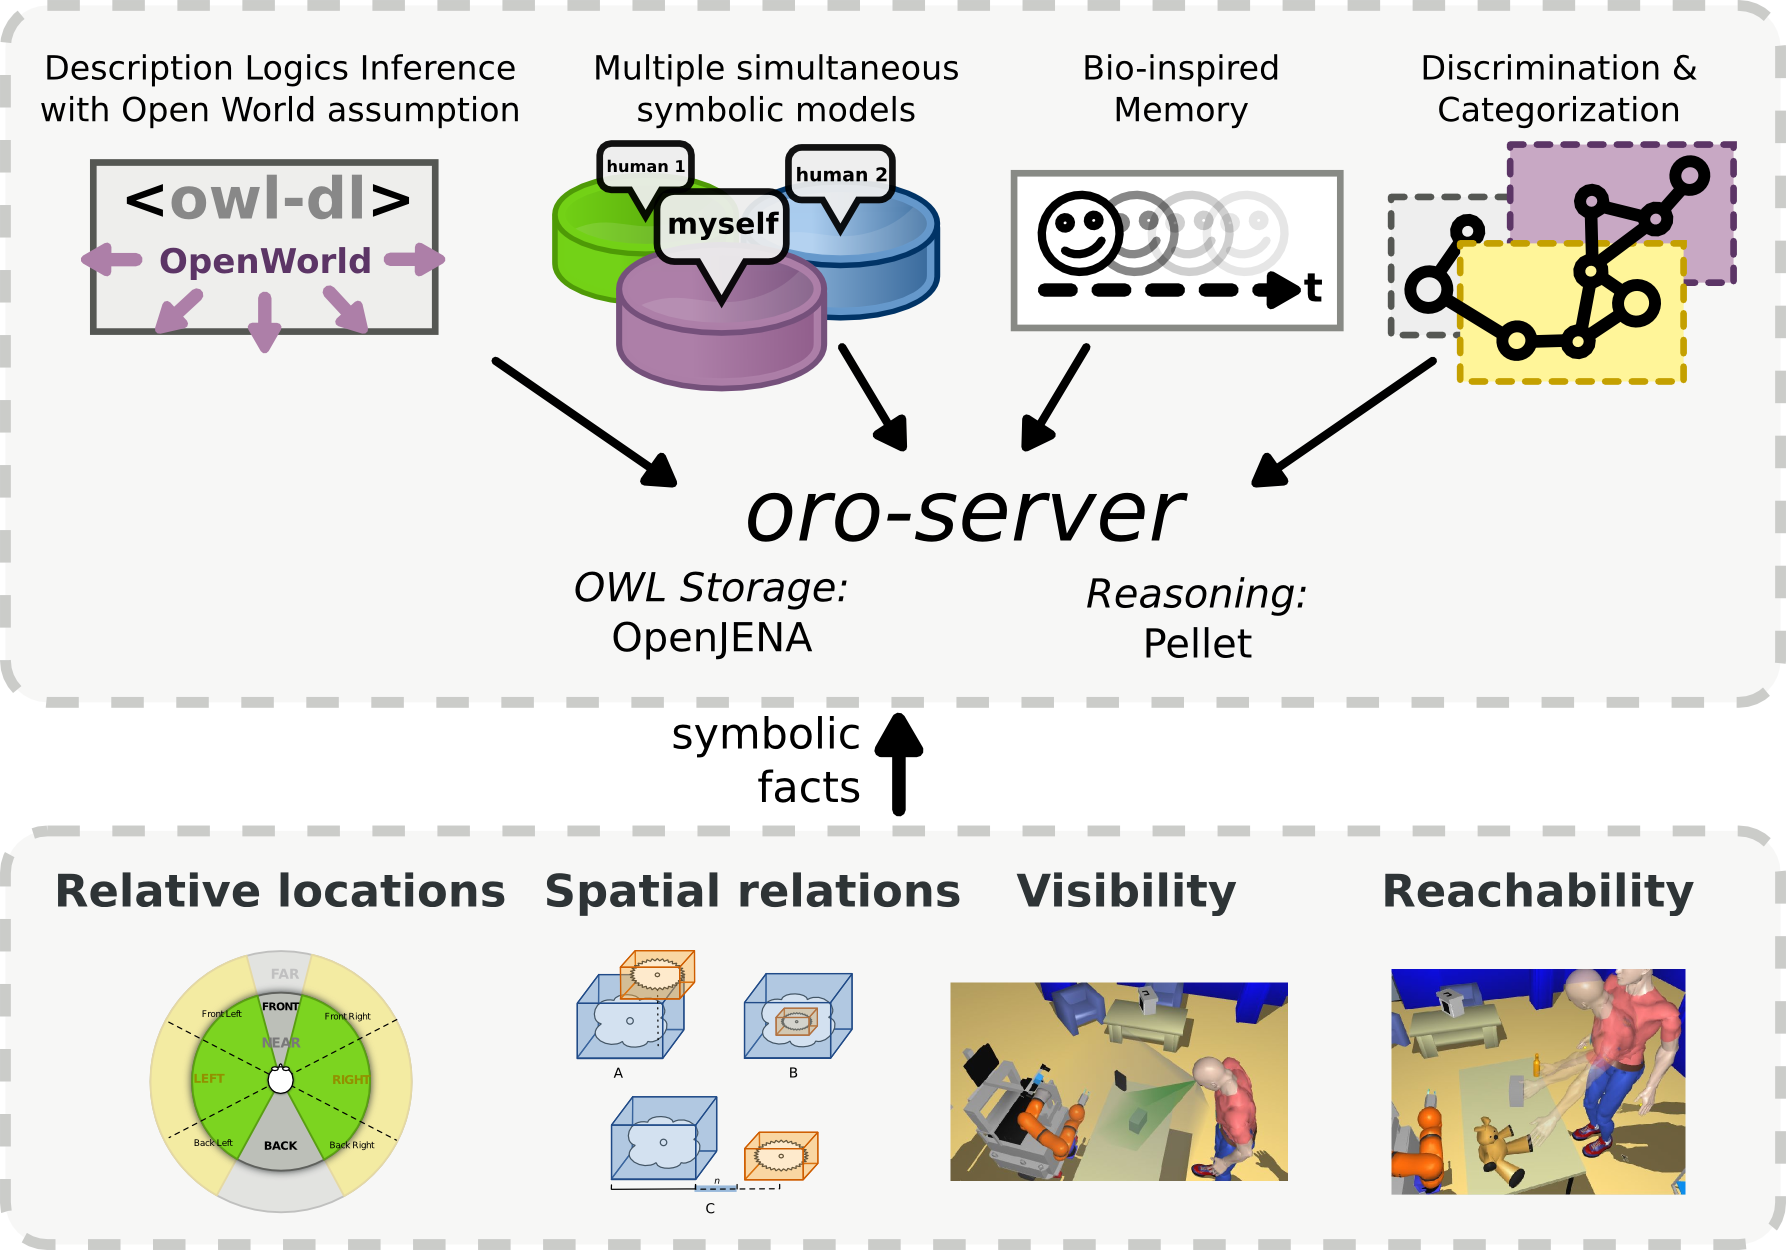
\includegraphics[width=\columnwidth]{spark-oro.png}
    \caption{Functional overview of knowledge base ({\sc Oro} server, top part) and the geometric situation assessment module (\emph{SPARK}, bottom part)}
        \label{fig|spark-oro}
\end{figure}

Anchoring perceptions in a symbolic model requires perception abilities and
their symbolic interpretation. We rely on a dedicated geometric and temporal
reasoning module called SPARK (\emph{SPAtial Reasoning \&
Knowledge}~\cite{Sisbot2011}). It is a situation assessment reasoner that
generates symbolic knowledge from the geometry of the environment with respect
to relations between objects, robots and humans (Fig.~\ref{fig|spark-oro}),
also taking into account the different perspective that each agent has on the
environment.

SPARK is an \emph{amodal} geometric model of the environment that serves both
as basis for the fusion of the perception modalities and as bridge with the
symbolic layer. This geometric model is continuously updated at run-time by the
robot based on its sensors (in our experiments, objects are identified and
localised through 2D barcodes, while humans are tracked with Kinect-like
devices, optionally assisted by motion capture to accurately track the head
motion, which is required to compute what the human is looking at).

\paragraph*{Computed symbolic relations} Over twenty physical relations are
continuously computed by SPARK: spatial relations, both agent-independent (like
\concept{isOn}, \concept{isNextTo} or \concept{isMoving}), and agent-dependent
(like \concept{isNear}, \concept{leftTo}), and also affordances:
\concept{sees}, \concept{looksAt}, \concept{pointsAt}, \concept{canReach}.
Visibility (with two levels corresponding to the field of view and the field of
attention) and pointing are computed by placing virtual cameras in the SPARK 3D
model, while reachability relies on inverse kinematics. Several filters (based
on hysteresis, expected object behaviour, etc.) allow to partially account for
perception noise~\cite{Warnier2012a}.

\paragraph*{Ego-centric and allo-centric frames} SPARK enables
\emph{perspective-taking}: spatial relations between entities can be computed
from different viewpoints, which let the robot build a different,
\emph{perspective-aware} symbolic model of the environment for each agent it
interacts with. These models are separately stored in the knowledge base.

This allows us to deal with ambiguities that arise when one speaker refers to
an object within a reference system (or changes the reference system, \ie
switches perspective) without making the reference frame
explicit~\cite{Breazeal2006, Ros2010}.

As a result, the robot stores models of the environment either in the
\emph{ego-centric} reference frame (from the robot perspective) or in the
\emph{allo-centric} frame (addressee-centred).


%%%%%%%%%%%%%%%%%%%%%%%%%%%%%%%%%%%%%%%%%%%%%%%%%%%%%%%%%%%%%%%%%%%%%%%%%%%%%%%%
\section{Communication}
\label{sect|com}

\paragraph*{Natural language grounding}

Natural language processing is one of the fields of human-robot interaction
for which the introduction of the semantic layer has been most beneficial.
In~\cite{Lemaignan2011a} we detail the techniques and the tool called
\texttt{dialogs} that we have developed for natural English language parsing and
grounding, along with verbalisation and (minimalist) dialogue management.

Natural language input (in experiments, we rely on an Android-based interface,
with Google speech recognition) is parsed into a grammatical structure, and
atoms of each sentence are resolved with the help of the ontology to ground
concepts like objects (\ie when a user says ``pick the can'', resolve to which
instance of \emph{can} the user is referring to) and actions. Sentences are
sorted into questions, desires and statements, and processed accordingly.

The system supports quantification (``give me \{a | the | some | all | any |
...\} can''), thematic roles (action-specific predicates that qualify the
actions), interactive disambiguation (the robot asks questions when it needs
more information), anaphora resolution (``give \emph{it} to me'') based on
dialogue history. It also permits knowledge extension by learning new semantic
structures (for instance, a sentence like ``learn that cats are animals'' is
converted into \stmt{Cat subClassOf Animal}), interprets common temporal and
place adverbs (like \emph{above} or \emph{tomorrow}) and translates to a
certain extend \emph{states} (``I'm tired'') into \emph{experiences}
(\stmt{HUMAN experiences state\_1, state\_1 hasFeature tired}).

\paragraph*{Limits of disambiguation at semantic level}

One prototypical example of semantic disambiguation has been given in
\cite{Ros2010b} with the child game \emph{spygame}: two players are facing
each other with a set of random objects in-between, one player mentally choose
one object, and the other player has to guess the object by asking closed
questions like \emph{Is your object small or large?} Based on the knowledge it
has acquired, the robot is able to minimize the number of questions required to
find the object.

When playing this kind of game, however, the issue arises that the robot has no
way to select which knowledge about the object is relevant in the interaction
context. For instance, the knowledge base may store facts like \stmt{obj1 type
ActiveConcept} (which internally means that this concept was mentioned in a
discussion in the last few seconds): this information is not a relevant
property of \concept{obj1} when trying to disambiguate concepts with humans.
This distinction between \emph{internal knowledge} (meaningful to
the system only) and \emph{common knowledge} (whose meaning is understood by
all the interactors) has not been properly dealt with in our architecture.

Besides, even knowledge that belongs to the \emph{common knowledge} may not be
appropriate in a given interaction context. For instance, the system may
compute that at a given instant the human is looking at the object: \stmt{human
looksAt obj1}. This property makes sense to both parties, but in the context of
the \emph{spygame}, we would like to mainly use immanent properties, not
volatile like a gaze. More research is required to identify relevant
interaction contexts and knowledge classes attached to them.

\subsection{Multi-modal communication}

Because all components rely on the same RDF formalism to format their outputs,
the different communication modalities (\emph{explicit} like verbal, deictic or
based on gaze, or \emph{implicit} like postures) are presented in a homogeneous
way. The dialogue grounding process makes use of them at two distinct levels.

First, particular steps of the grounding process explicitly check for the
presence and value of specific facts: for instance, when a set of instances
matches a category (the human says ``give me the bottle'' and the robot knows
about three bottles), the module may decide (it actually depends on the
quantifier preceding the class) to discard some of them based on their
\emph{visibility} for the speaker (implicit communication context built on the
human posture).

Another example, when the human says ``this'', the robot checks if the human is
currently pointing at some object. In that case, \emph{this} is replaced by the
object focused on.

Note that, while the system benefits from the complementary modalities, they
are not all required. The dialogue system would for instance happily run with
only the verbal modality, at the cost of weaker interaction.

The second level of integration of multi-modality is implicit: by computing
symbolic properties from the geometry, richer descriptions and hence
discrimination possibilities are available: for instance, if reachability is
available, the robot may ask ``do you mean the bottle that is accessible to
me?'' to discriminate between the three bottles. That way, procedures relying
on discrimination transparently benefit from added modalities.

%%%%%%%%%%%%%%%%%%%%%%%%%%%%%%%%%%%%%%%%%%%%%%%%%%%%%%%%%%%%%%%%%%%%%%%%%%%%%%%%
\section{Robot control}
\label{sect|ctrl}

\subsection{Desires and experiences}

Our robot execution controllers (OpenPRS-based {\sc Shary} or Python-based {\sc
pyRobots}) have deep integration with the knowledge base. It serves as the
primary source of information for semantic-aware decision-making.

We split the interaction situations stemming from the situation assessment and
communication components in two categories: \emph{desires} (performative act)
and \emph{experiences} (assertive act).

\emph{Desires} are typically human orders (``Give me that book''). The nature
of the desired action (to pick, give, look, bring, show...), along with the
action parametrization (what is acted on? who should perform the action? etc.)
are extracted from the knowledge base, and either passed to a task planner
(presented in the next section) or executed if the procedure is directly
available.

\emph{Experiences}, on the other hand, comprise of emotions, states and
questions (when asking a question, we consider the human to be in an
\emph{interrogative state}). When the knowledge base recognizes that an agent
\emph{experiences} a particular emotion or state, the execution controller may
decide to handle it, typically by trying to answer the question or using the
emotional or physical state as a parameter for subsequent actions. As an example,
when the speaker says ``I feel tired'', we change the motion planner
parametrization to lower the effort the human needs to provide for the following
joint manipulation tasks. Note that this example has been implemented as a
proof-of-concept. We have not yet tried to define a theoretical framework that
would support action alteration based on the user's experienced states.

\subsection{Event-driven control}

The {\sc Oro} server proposes two paradigms to access its content: RPC-style
queries (based on the standard SPARQL language) or events. In its simplest
form, a module can subscribe to an event by passing through an event pattern
(in its basic form, a partial statement like \stmt{? type Elephant}) and a
callback.  Each time a new instance of elephant appears in the knowledge base,
the callback is triggered.

This allows us to write reactive robot controllers with a high level of
expressiveness: for instance, by subscribing to the event \stmt{human1 desires
?action, ?action type Look, ?action hasGoal myself}, we could trigger a
behaviour when the human expresses (through dialogue, gestures...) that he
wants to look at the robot itself.

The robot controller designer does not need to directly care about how this
\emph{desire} is produced (this is delegated to perception modules), he can
focus on the semantic of the desire.

Note also that we take advantage of the reasoning capabilities of the system:
for example, the goal of the action (\stmt{action hasGoal myself}) may not be
explicitly asserted, but inferred by the reasoner based on other assertions.

\subsection{Task planning}

Our execution controllers rely on symbolic task planning to convert faraway
desires into a succession of atomic actions. We use in our architecture the
HATP planner (for Human Aware Task Planner~\cite{Alili2009}).  HATP is based on
a Hierarchical Task Network (HTN) refinement, which performs an iterative task
decomposition into sub-tasks until reaching atomic actions. The \emph{planning
domain} defines the set of methods describing how to decompose a task and
represents the procedural knowledge of the robot.

In order to produce a collaborative behaviour, the robot plans not only for
itself but also for the other agents. The planning domain of each agent is
instantiated from the agent-specific model in the {\sc Oro} server. The resulting
plan, called \emph{shared plan} is a set of action streams, one per
agent involved in the goal achievement. HATP can also be tuned by setting up
different costs depending on the actions to apply and by taking into account a
set of constraints called \emph{social rules}. This tuning aims at adapting the
robot's behaviour according to the desired level of cooperation of the robot.

Two important remarks: because HATP is a generic symbolic task planner, we have
been able to design a planning domain at a semantic level which is close to the
one used in the human-robot dialogue (the planner vocabulary contains concepts
like \texttt{give}, \texttt{table}, \texttt{is on}...). Hence only a few
ontology rules have been required to map both the knowledge extracted from the
situation assessment and the statements originated from the verbal interaction
to the planner domain.

Second remark, after some research (see appendix B of~\cite{Lemaignan2012a} for
a detailed discussion)  we have decided to represent neither the planning
domain nor the resulting plans in the knowledge base: the planning domain (with
task pre- and postconditions) is stored in a specific format, outside of the
central declarative knowledge repository, and the plans are directly
communicated to the robot controller. Thus, like many other cognitive
architectures, we have independent declarative and procedural knowledge stores.

%%%%%%%%%%%%%%%%%%%%%%%%%%%%%%%%%%%%%%%%%%%%%%%%%%%%%%%%%%%%%%%%%%%%%%%%%%%%%%%%
\section{Internal cognitive processes}
\label{sect|intern}

\subsection{Theory of Mind}
\label{sect|tom}

Theory of Mind (originally defined in~\cite{Premack1978}) is the cognitive
ability that a subject possesses to represent the mental state of another
agent, possibly including knowledge that contradicts the subject's own model: for
example, a book can be at the same time \emph{visible} for myself, and \emph{not
visible} for you.

Children develop this skill, which is essential to understand others' perspectives during
interactions, around the age of three. It supposes the
ability to build, store and retrieve separate models of the knowledge of the
interactors.

Our knowledge base implements such a mechanism: when the robots infers a new
agent has been introduced in the knowledge base, it initializes a new,
independent, ontology for this agent. All the ontologies that are created share
the same common-sense knowledge, but rely on each agent's perspective for the
actual instantiation: the robot (geometrically) computes that the book is in
its own field of view, but not in the human one. The robot knowledge contains
the fact \stmt{book isVisible true} while the human model contains \stmt{book
isVisible false}.

One classical application of this cognitive skill is the so-called
\emph{False-Belief} experiment (also known as the \emph{Sally and Ann}
experiment)~\cite{Leslie2000}: a child is asked to watch a scene where two
people, A and B, manipulate objects. Then A leaves and B hides away one
object. When A comes back, we ask the child ``where do you think A will
look for the object?''. Before acquiring a theory of mind, children are not
able to separate their own (true) model of the world (where they know that
the object was hidden) from the model of A, which contains \emph{false
beliefs} on the world (A still thinks the object is at its original
position since he did not see B hiding it). Using separate knowledge models
in the knowledge base, we have been able to replicate this experience with
our robots~\cite{Warnier2012a}.

\subsection{Working memory}

The {\sc Oro} server also features a mechanism to mimic minimalistic forms of
biological memory.  When new statements are inserted in the knowledge base, a
\emph{memory profile} is optionally attached to them.

Three such profiles are predefined: {\tt short term}, {\tt episodic} and {\tt
long term}. They each correspond to a different lifetime for the statements
(respectively 10 seconds, 5 minutes and no time limit). After this duration,
the statements are automatically removed from the knowledge base.

This approach is limited. In particular, \emph{episodic} memory primarily
refers to the semantics of the statements (that is expected to be related to an
event) and not to a specific life duration.

We rely however on this short term memory for a particular use-case:
\emph{active concepts}. Some modules, like the natural language processor, use
the {\tt short term} memory profile to mark for a few seconds important
concepts that are currently manipulated by the robot. For example, if a human
asks the robot: ``Give me all red objects'', the human, the \concept{Give}
action, and each red objects that are found are successively marked as
\emph{active concepts} by inserting statements such as \stmt{human type
ActiveConcept} in the short-term memory (which can be considered, in this case,
to be a working memory). We use this feature to trace certain knowledge-related
processes.

\subsection{Cognitive activity}

\begin{figure}
        \centering
        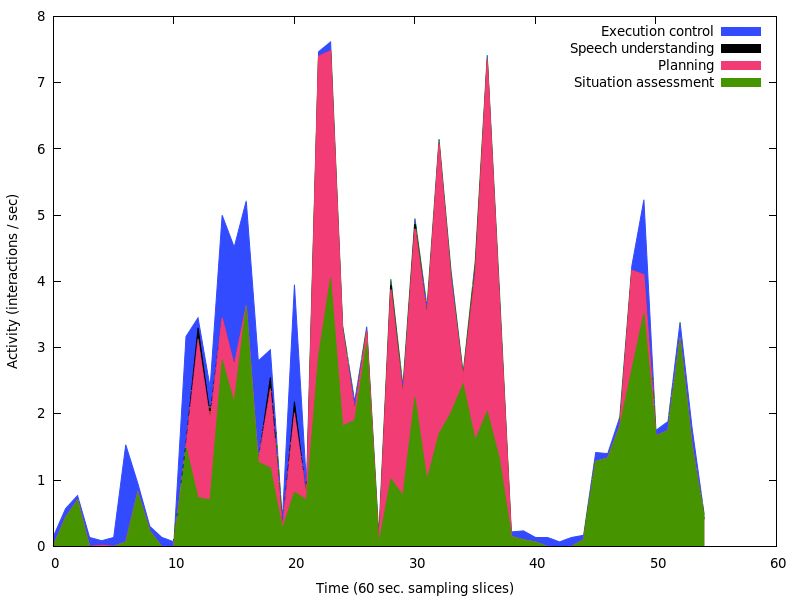
\includegraphics[width=\columnwidth]{figs/cognitive_load.png}
        \caption{This diagram shows the average number of interactions with the
        knowledge base during a one-hour long experiment with the robot.
        Interactions are either knowledge alteration (addition/removal of
        statements) or queries. They are averaged on a sliding window of 60 seconds.}
        \label{fig|cognitiveload}
\end{figure}

Fig.~\ref{fig|cognitiveload} is a plot of the interactions (knowledge
alterations or knowledge queries) between the robot's modules and the central
knowledge base during a one-hour long experiment. Because most of the
communication between the modules are in fact supported by the knowledge base in
our architecture (Fig.~\ref{fig|archi}), it reflects well the exchanges of
semantic informations within the deliberative layer of the robot, which we can
tentatively call the \emph{cognitive activity} of the robot.

This simplistic measurement needs to be refined to take into account the fact
that the raw number of RPC calls to the knowledge base only imperfectly
reflect the actual cognitive processes running on, but it opens interesting
perspectives nevertheless. We could for instance investigate possible
correlations with the cognitive activity of a human partner (measured via EEG
or qualitative feedback).



%%%%%%%%%%%%%%%%%%%%%%%%%%%%%%%%%%%%%%%%%%%%%%%%%%%%%%%%%%%%%%%%%%%%%%%%%%%%%%%%
\section{Discussion}
\label{sect|conclusion}

Altogether, the components we have presented compose an architecture that we
call \emph{knowledge-oriented}:

\begin{itemize}
    
    \item{Knowledge is explicitly stored in one central and consistent
    repository of facts, accessible for all modules.} 

    \item{Knowledge is represented in a strict formalism (OWL statements) and
    with a clearly defined vocabulary (stated in the common-sense ontology).}

    \item{The first two points enable a loosely-coupled architecture where
    modules can be removed or replaced easily by other ones as long as
    they share the same semantics (modules are defined by the knowledge they
    produce),} 

    \item{We adopt a \emph{symbolic}, reactive, event-driven approach to robot control.
    By managing events at the same level as the reasoner, we take full
    advantage of the inference abilities of {\sc Oro} to trigger events whose
    \texttt{true} conditions can be inferred.} 

    \item{Finally, this architecture allows for the combination of very
    different knowledge modalities in a single homogeneous environment,
    bringing mutual benefits to components. For instance, the dialogue
    processing module can perfectly run without any geometric
    perception, but its disambiguation routines can transparently
    benefit from it when available (since richer symbolic descriptions of
    objects are then available).}

\end{itemize}

Those items are not new \emph{per se}. It seems however interesting to
underline the shift of focus this implies during the design and integration
phases. We can adopt three perspectives to discuss the techniques we have
presented here: first, the \emph{architect perspective}: what are the pros and
cons of our approach from an engineer's point of view. Then, the \emph{logician
perspective}: does the promises of automated reasoning for robots really come
to fruition with ontologies? And finally the \emph{cognitician perspective} or
how explicit knowledge manipulation endows our robots with new cognitive
capabilities.

\subsection{The Architect view: loose coupling and modalities merging}

In this article, we have presented several sub-systems of our robots: a module for geometric
reasoning and situation assessment (written in C++), a natural
language interface (written in Python), a symbolic task planner (written in
C++), two execution controller (one written in Python, one in PRS). These
modules communicate together through RDF statements with only a few exceptions.

Since these statements are anchored in the robot's pool of knowledge, they
actually convey shared and unambiguous \emph{meaning} through the system. This
has one important consequence from the perspective of the system architecture:
interfaces between modules are only defined in terms of knowledge consumption and/or
production. This brings good decoupling properties. For instance, the output of
the dialog module is a new \emph{situation desired} by the speaker. This module
can be transparently replaced or completed by any other module that produces
the same chunks of knowledge. Only a thin protocol layer remains to get the
modules to interact with each other. This allows us to implement (otherwise difficult)
merging of radically different perception modalities like vision (the robot
sees an object on a table: the output would look like \stmt{obj1 isOn table1})
and verbal description (a human says to the robot the object on the table
is red: it leads to a query \stmt{? isOn table1} and then a new assertion:
\stmt{obj1 hasColor red}).

Another consequence is that the communication channels are {\it
de facto} defined by the semantics of the information they
convey. This allows the system designers to think in terms of which module
produces or needs which knowledge, instead of which module produces which
service. We found this approach to be helpful when implementing cognitive
functions like the theory of mind, the perspective taking or the natural
language grounding.

Finally, another good property of knowledge-based communication between modules
is the \emph{cognitive observability} of the system: by logging queries between
modules (which is even easier in our case since we rely on a central knowledge
management), one can trace the interactions between the robot subsystems at a high
abstraction level. We address the significance of this property
from the cognitive point of view below.

The knowledge-oriented architecture also has shortcomings. We can name here a few.

Because the sources of knowledge the robot has to deal with are multiple and
often not known at startup (typically, the knowledge generated by a verbal
interaction with a human), it is difficult to formally guarantee reliability.

Also, it must be noted that actuation itself is directly piloted by the
execution controller through standard RPC calls (ROS actions and/or Pocolibs
requests): no knowledge abstraction takes place.

Also on the sensing side, we have to bypass the semantic layer in certain cases
(extension of the symbolic task planner with geometric constraints is one
example).

Many aspects like uncertainty management, modal logics,
non-monotonic reasoning are not well addressed with the Description Logic
formalism, and remain to be explored to gain the level of expressiveness
required to cover many of the more complex human-robot interaction scenarios.

\subsection{The Logician view: the importance of trivial inferences}

\begin{quote}

    Where to find milk? Milk is a subclass of dairy which is itself a subclass
    of a perishable goods. The usual storage place for perishable goods is the
    fridge, so the milk is likely to be found in a fridge.

\end{quote}

This example of reasoning, quoted from Moritz Tenorth, is a good example of
simple yet non-trivial reasoning. As a matter of fact, only very few of such
prototypical reasoning cases were positively identified in our scenarios and experiments
(and consequently implemented as rules in {\sc Oro}).

The design choices of our architecture partially explain that fact: first, the
planning task (which is a typical reasoning task) is delegated to a
dedicated, external planner (HATP). Then, time is not represented in {\sc Oro}, and
consequently no temporal reasoning takes place at this level: action
recognition or monitoring are handled by other layers, and the underlying
reasoning tasks are not implemented as explicit symbolic rules in the knowledge
base.

The experiments we have conducted are also likely to have too simplistic
semantics to let complex reasoning needs emerge. Scenarios with more complex
semantics would be desirable to better stress the expressiveness and inference
abilities provided by Description Logics.

Is reasoning at the knowledge level immature or even superfluous, then? Not so:
hundreds of trivial (from a human point of view) inferences are continuously
produced by the system (translating inheritance relations, domain/range
constraints, transitivity, etc.) and encode a large amount of common-sense
knowledge that can not be otherwise conveniently asserted. These trivial
inferences are all the more important that an expressive knowledge
representation language is used. Since a language like OWL allows it to
directly represent high-level concepts like partitions, cardinality
restrictions, properties' ranges and domains, it leads to a more
\emph{implicit} description of the available knowledge.  This in turn pushes
for a lot of ``trivial'' reasoning to make the knowledge pool explicit, and
hence largely reusable by the deliberative subsystems. With the progress in the
understanding of the relations between expressiveness and (tractable)
satisfiability, along with the progress of reasoners, more and more of the
assertions do not need to be explicit anymore, and consequently are delegated
to the reasoner.

We think that \emph{common-sense encoding} is likely to remain the main
application of reasoning in our architecture, where reasoning related
to decision making mostly happens outside the knowledge representation system.


\subsection{The Cognitician view: palpable knowledge and semantic thinking}

The original motivation to introduce explicit knowledge management in our
architecture was to transform the knowledge in the robot from some ubiquitous,
pervasive, multi-modal and, most importantly, mostly undefined feature of the
system into an observable, quantifiable, manipulable resource: a
\emph{palpable} feature of the system.

This transformation, both from the technical point of view (the {\sc Oro}
server, the ontologies, the bindings, etc.) and as a more subtle change in the
practises related to the development of robotic components, is probably the
main outcome of this work.

Knowledge is not an abstract concept anymore: it is a set of statements, in
most cases directly intelligible to the developers, stored in one place. We can
export them, monitor them, review them, question them.

Communication between the robot's modules is now conceived in terms of what are
the \emph{semantics} of the information flows, instead of a simple
compatibility of interfaces. When defining the frontiers of a robotic
component, we do not think anymore only in terms of \emph{is the interface complete
and self-contained}, but also in terms of \emph{is the semantic complete and
consistent?}. This allows a deeper, more correct modularity: two modules that
share the same, well-defined semantic can be confidently exchanged. When we
remove or disable a component (the dialogue processing, the geometric
reasoning, ...), we know precisely what knowledge will not be available
anymore.

We call this new property of our robot, that allows for both qualitative and
quantitative analysis of the beliefs, its \emph{cognitive observability}.

It is somewhat related to the idea of \emph{cognitive penetrability} introduced
by Pylyshyn~\cite{Pylyshyn1989} in 1989, in the context of the study of
possible strong equivalences between computational models and the
\emph{psychological reality}:

\begin{quote}

    [One of the criterion] relies on the assumption that we can identify
    certain clear cases of phenomenon that should be accounted for at the
    knowledge level, that is, in terms of the representations alone, rather
    than in terms of properties of the cognitive architecture. Phenomena that
    depend in a rational way on subjects' goals, beliefs, and utilities are a
    case in point. For example in psychophysics we assume that if a measure
    (such as a threshold) changes systematically as we change the payoffs (that
    is, the relative cost of errors of commission and of omission), then the
    explanation of that change must be given at the knowledge level -- in terms
    of decision theory -- rather than in terms of properties of sensors or
    other mechanisms that are part of the architecture. In general showing that
    certain empirical phenomena are sensitive to goals and beliefs (or what I
    call \emph{cognitively penetrable}) is prima facie evidence that they
    should not be attributed to properties of the architecture.

\end{quote}

The introduction of an explicit \emph{knowledge level} in our architecture
makes it possible to effectively assess the cognitive penetrability of the
whole robot behaviours (this is however not new, and traditional BDI
architectures would also make this claim).

Even more, this architecture also contributes to bring closer robotics and
cognitive psychology: it provides clear entry points to implement some
classical psychology tests to robots, be it related to perspective taking, to
language understanding, to a theory of mind (such as the \emph{False-Beliefs}
experiment), etc.

\section{Conclusion}

This article does not claim to provide an exhaustive assessment of the
strengths and weaknesses of explicit knowledge management in a large robotic
architecture. Most of the ``lessons'' that we have ``learned'' are not new, and
the various scientific communities (task planning, architecture control, NLP,
geometric reasoning, social psychology...) that are related to human-robot
interaction and robotic cognition already know them.

One of the difficult challenges of cognitive robotics, however, is to overcome
the relative isolation of each of these communities to build an autonomous
embodied agent, able to interact with humans. This contribution modestly offers
a critical look at one instance of such a ``real-world'' robotic architecture,
that tackles several of the facets of cognitive robotics.

If we had a single ``lesson'' to retain, it would likely be that one: shifting
from a robotic design based on \emph{modules and APIs} to a system based on
\emph{modules and human-level semantic interfaces} has been the main
facilitator both for glueing together heterogeneous deliberative modules in a
\emph{meaningful} way, and quickly developing prototypes for new
upper-cognition abilities, like natural dialogue and theory of mind.

\section*{Acknowledgment}

This work has been supported by EU FP7 ``SAPHARI'' under grant agreement no. ICT-287513.

\bibliographystyle{IEEEtran}
\bibliography{IEEEabrv,biblio}


\end{document}
